% LTeX: language=pl-PL
\chapter{Podstawy matematyczne}\label{ch:podstawy}
\section{Liczby zespolone}
Czy~widział ktoś kiedyś liczbę? Na~przykład takie czterdzieści
dwa\footnote{Zobacz: Douglas Adams, ,,Autostopem przez~Galaktykę''.}? Czy można ją
zobaczyć? Możemy zobaczyć reprezentację liczby czterdzieści dwa w~postaci zapisu
dziesiętnego
\begin{quotation}
	\centering 42\index{forty two},
\end{quotation}
lub~binarnego
\begin{quotation}
	\centering 101010,
\end{quotation}
możemy też~zobaczyć czterdzieści dwa obiekty -- na~przykład ręczniki.
Jednak samej liczby zobaczyć nie~możemy, bo jest ona pojęciem abstrakcyjnym, które
istnieje niezależnie od~reprezentacji czy~interpretacji. Liczba czterdzieści dwa
jest liczbą naturalną. Tak samo jest z~liczbami wymiernymi i~rzeczywistymi ---
nie~możemy ich zobaczyć, dotknąć czy~powąchać; jednakże możemy na~nich działać.

Powyższe wprowadzenie ma Cię przekonać, że~liczby zespolone, o~których zaraz
będzie mowa, nie~są straszniejsze, dziwaczniejsze czy~bardziej abstrakcyjne
niż~liczby naturalne, całkowite, wymierne czy~rzeczywiste.
Dla~matematyka liczby są pewnymi obiektami, które mają pewną (mniej lub~bardziej elegancką)
strukturę matematyczną, między którymi istnieją relacje i~na~których można wykonywać pewne działania.
Dla~fizyka czy~inżyniera natomiast liczby służą do~opisu rzeczywistości:
naturalne -- do~zliczania obiektów, wymierne -- do~opisu stosunków między licznościami,
rzeczywiste -- do~mierzenia czasu, odległości, siły, a~zespolone -- do~opisywania prądu zmiennego,
fal lub~mechaniki kwantowej. Liczby zespolone stosowane są często tam, gdzie~mamy do~czynienia
z~obrotami lub~cyklicznie zmieniającymi~się wartościami.

Przejdźmy zatem do~rzeczy: zdefiniujmy liczby zespolone i~działania, jakie można
na~nich wykonywać.
Na~początek wprowadźmy jednostkę urojoną: ,,$\i$'', czyli~taką liczbę, dla której $\i^2=-1$.
Teraz możemy powiedzieć, że~\newterm{liczbą zespoloną}\index{liczba zespolona}
możemy nazwać dowolną liczbę $z$ taką, że
$$
	z = a + b \i,
$$
gdzie $a$ i~$b$ są liczbami rzeczywistymi. Samą liczbę $a$ nazywamy
\newterm{częścią
	rzeczywistą}\index{liczba zespolona!część rzeczywista} $z$ i~oznaczamy ją przez~$\Re z$,
a~$b$ nazywamy \newterm{częścią urojoną} \index{liczba zespolona!część urojona}
liczby $z$ i~oznaczamy przez~$\Im z$.
Zbiór liczb zespolonych oznacza~się przez~$\Complex$. Oznaczamy, że~$z$ należy do~zbioru~$\Complex$
-- albo~inaczej: że~jest liczbą zespoloną -- pisząc $z\in\Complex$.

Liczby zespolone przedstawia~się na~tzw.~płaszczyźnie zespolonej, na~której
na~osi poziomej odkłada~się wartość części rzeczywistej, a~na~osi pionowej -- wartość części urojonej.

\subsubsection{Moduł i~argument liczby zespolonej}
W~przypadku liczby zespolonej możemy mówić o~dwóch jej własnościach: module i~argumencie.
\newterm{Moduł liczby zespolonej}\index{liczba zespolona!moduł} zadany jest~-- jak
w~twierdzeniu Pitagorasa -- jako
$$
	\abs{z} = \abs{a+b\i} = \sqrt{a^2+b^2}.
$$
Należy zauważyć, że~moduł liczby zespolonej jest rzeczywisty i~zawsze większy lub~równy
zero. Moduł rozumiemy jako odległość liczby $z$ od~liczby $0=0+0\i$.

\newterm{Argumentem liczby zespolonej}\index{liczba zespolona!argument}
$z = a + bi \neq 0 + 0\i$ nazywamy liczbę rzeczywistą $\phi$ z~przedziału $[0,2\pi)$ spełniającą układ równań
$$
	\cos \phi = \frac{a}{\abs{z}}  \text{ oraz }   \sin \phi=\frac{b}{\abs{z}}.
$$
Inaczej można powiedzieć, że~argument liczby $z$ to wyrażona w~radianach wartość
kąta skierowanego $\phi$ pomiędzy osią rzeczywistą a~półprostą poprowadzoną od~środka układu
współrzędnych i~przechodzącą przez~punkt będący graficzną reprezentacją liczby $z$.
Ilustracją do~powyższych definicji jest Rysunek~\ref{rys:postaćgeometryczna}.

\subsubsection{Wzór Eulera}
Dla~liczby rzeczywistej $\phi$ możemy zapisać następującą relację, nazywaną wzorem Eulera\footnote{
	Leonhard Euler szwajcarski matematyk i fizyk (1707 -- 1783).}:
$$
	e^{\i \phi} = \cos\phi + \i \sin\phi.
$$
Zauważmy, że~dla~każdego $\phi\in \Real$ moduł liczby $|e^{\i \phi}| = 1$.

\subsubsection{Postać trygonometryczna liczby zespolonej}
Liczbę zespoloną $z = a + b\i \neq 0 + 0\i$ można zapisać w~postaci trygonometrycznej
$$
	z = \abs{z}(\cos \phi + \i \sin \phi),
$$
gdzie~$\phi$ jest argumentem liczby zespolonej.
Jeśli skorzystamy ze~wzoru Eulera, możemy zapisać liczbę $z$ jako
$$
	z = \abs{z}e^{\i \phi}.
$$
Warto dodać, że~w~fizyce moduł liczby nazywany jest często \newterm{amplitudą}\index{liczba zespolona!amplituda},
a~argument -- \newterm{fazą}\index{liczba zespolona!faza}.

\begin{figure}[h]
	\centering
	\resizebox{2in}{!}{
		\begin{tikzpicture}
			\begin{scope}[thick,font=\normalsize]
				\draw
				(3,0) coordinate (a) node[above right] {$\Re z$}
				-- (0,0) coordinate (o)
				-- (0,4) coordinate (b) node[above right] {$\Im z$}
					[->] (0,0) -- (3,4) coordinate (z) node[above right] {$z$} node [above=6pt, midway]  {$\abs{z}$}
				pic["$\phi$", draw=black, ->, angle eccentricity=1.2, angle radius=2cm]
					{angle=a--o--z};
				\draw (3,0) -- (3,4) [dashed, thin];
				\draw (0,4) -- (3,4) [dashed, thin];

				\draw [->] (-1.1,0) -- (5,0) node [above left]  {};
				\draw [->] (0,-1.1) -- (0,5) node [below right] {};

				\foreach \n in {-1,...,-1,1,2,...,4}{%
						\draw (\n,-3pt) -- (\n,3pt)   node [below=5pt] {$\n$};
						\draw (-3pt,\n) -- (3pt,\n)   node [left=1ex] {$\n \i$};
					}
			\end{scope}
		\end{tikzpicture}
	}
	\caption{Płaszczyzna zespolona. Liczba zespolona $z=3+4\i$
		znajduje~się na~końcu strzałki. Moduł liczby $z$, oznaczony jako $|z|$,
		to długość strzałki. Wynosi on $\sqrt{3^2+4^2}=5$. Natomiast
		argument jest oznaczony jako $\phi$ i~wynosi $\arccos{\frac{3}{5}}\approx 0{,}92\ \mathrm{rad}.$}
	\label{rys:postaćgeometryczna}
\end{figure}

\subsubsection{Sprzężenie liczby zespolonej}
\newterm{Sprzężeniem liczby zespolonej}\index{liczba zespolona!sprzężenie} $z = a + b\i$ jest liczba
$$
	\conj{z} = a - b\i.
$$
Sprzężenie geometrycznie może być rozumiane jako odbicie symetryczne liczby wokół osi rzeczywistej.

\subsubsection{Operacje arytmetyczne na~liczbach zespolonych}
Dodawanie i~odejmowanie liczb zespolonych przeprowadza~się w~sposób naturalny, tzn.
jeśli~dodajemy dwie liczby zespolone $z_1 = a_1 + b_1 \i$ oraz~$z_2 = a_2 + b_2 \i$, to
ich suma wynosi
$
	z_1 + z_2 = (a_1 + a_2) + (b_1 + b_2) \i,
$
a~ich różnica
$
	z_1 - z_2 = (a_1 - a_2) + (b_1 - b_2) \i.
$
Geometryczna interpretacja dodawania
liczb zespolonych jest podana na~Rysunku~\ref{rys:dodawaniezespolonych}.

\begin{figure}[b]
	\centering
	\subbottom[Dodawanie liczb zespolonych $z_1 = 2 + 1\i$ oraz $z_2 = 1 + \frac{3}{2}\i$.\label{rys:dodawaniezespolonych}]%
	{
		\resizebox{0.46\textwidth}{!}{
			\centering
			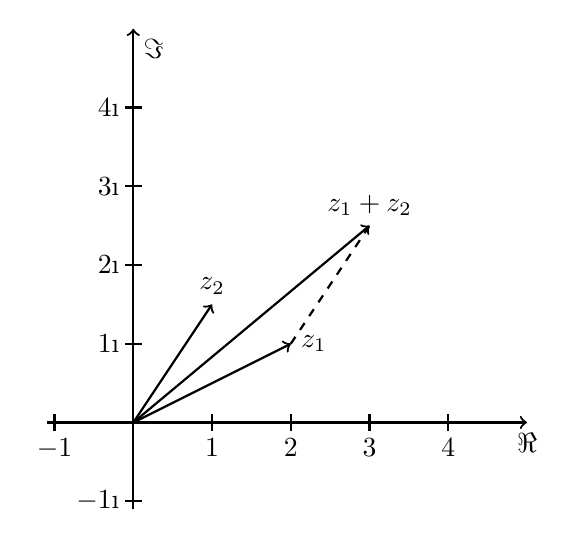
\begin{tikzpicture}
				\begin{scope}[thick,font=\normalsize]

					\draw [->] (-1.1,0) -- (5,0) node [below]  {$\Re$};
					\draw [->] (0,-1.1) -- (0,5) node [below right] {$\Im$};


					\draw [->] (0,0) -- (2,1) node [right]  {$z_1$};
					\draw [->] (0,0) -- (1,1.5) node [above]  {$z_2$};

					\draw  [dashed] (2,1) -- (3,2.5) ;
					\draw [->] (0,0) -- (3,2.5) node [above]  {$z_1+z_2$};

					\foreach \n in {-1,...,-1,1,2,...,4}{%
							\draw (\n,-3pt) -- (\n,3pt)   node [below=5pt] {$\n$};
							\draw (-3pt,\n) -- (3pt,\n)   node [left=1ex] {$\n \i$};
						}
				\end{scope}
			\end{tikzpicture}
		}
	}\hfill
	\subbottom[Mnożenie liczb zespolonych $z_1 = 3 + \frac{1}{2}\i$ oraz~$z_2 = 1 + 1\i$. Aby~uzyskać ich iloczyn, musimy pomnożyć amplitudy i~dodać fazy.\label{rys:mnożeniezespolonych}]%
	{
		\resizebox{0.46\textwidth}{!}{
			\centering
			\begin{tikzpicture}
				\begin{scope}[thick,font=\normalsize]

					\draw
					(3,0) coordinate (a)
					-- (0,0) coordinate (o)
					-- (0,0.5) coordinate (b)
					[->] (0,0) -- (3	,0.5) coordinate (z) node[right] {$z_1$} node [above, pos=0.65]  {$\abs{z_1}$}
					pic["$\phi_1$", draw=black, ->, angle eccentricity=1.2, angle radius=2cm]
						{angle=a--o--z};

					\draw
					(1,0) coordinate (a)
					-- (0,0) coordinate (o)
					-- (0,1) coordinate (b)
					[->] (0,0) -- (1,1) coordinate (z) node[above right] {$z_2$} node [above=0.15, midway]  {$\abs{z_2}$}
					pic["$\phi_2$", draw=black, ->, angle eccentricity=1.3, angle radius=1cm]
						{angle=a--o--z};

					\draw
					(0.5,0) coordinate (a)
					-- (0,0) coordinate (o)
					-- (0,3) coordinate (b)
					[->] (0,0) -- (-0.5,3) coordinate (z) node[above left] {$z_1 z_2$} node [left, midway]  {$\abs{z_1}\abs{z_2}$}
					pic["$\phi_1 + \phi_2$", draw=black, ->, angle eccentricity=1.2, angle radius=2.7cm]
						{angle=a--o--z};

					\draw [->] (-1.1,0) -- (5,0) node [below]  {$\Re$};
					\draw [->] (0,-1.1) -- (0,5) node [below right] {$\Im$};

					\foreach \n in {-1,...,-1,1,2,...,4}{
							\draw (\n,-3pt) -- (\n,3pt)   node [below=5pt] {$\n$};
						}
					\foreach \n in {-1,...,-1,1,2,...,3}{
							\draw (-3pt,\n) -- (3pt,\n) ;
						}
					\foreach \n in {4}{
							\draw (-3pt,\n) -- (3pt,\n)   node [left=1ex] {$\n \i$};
						}

				\end{scope}
			\end{tikzpicture}
		}
	}
	\caption{Graficzna reprezentacja dodawania i~mnożenia liczb zespolonych}
	\label{rys:dodawanieimnożeniezespolonych}
\end{figure}

Mnożenie i~dzielenie liczb zespolonych jest nieco mniej intuicyjne. Jeśli~dane
są $z_1$ i~$z_2$ takie jak powyżej, ich iloczyn wynosi
\begin{equation*}
	\begin{split}
		z_1 z_2 =&(a_1+b_1 \i) (a_2 + b_2 \i)=
		\\=&a_1 a_2 + a_1 b_2 \i + b_1 a_2 i - b_1 b_2 = (a_1 a_2 - b_1 b_2) + (a_1 a_2 + b_1 b_2)\i,
	\end{split}
\end{equation*}
a~ich iloraz wynosi
$$ \frac{z_1}{z_2} =
	\frac{a_1 + b_1\i}{a_2 +b_2\i} =
	\frac{\left(a_1 + b_1\i\right) \cdot \left(a_2 - b_2\i\right)}
	{\left (a_2 + b_2\i\right) \cdot \left (a_2 - b_2\i\right)} =
	\left({a_1a_2 + b_1b_2 \over a_2^2 + b_2^2}\right) \left( {b_1a_2 - a_1b_2 \over a_2^2 + b_2^2} \right)\i.
$$

Mnożenie i~dzielenie liczb zespolonych łatwiej objaśnić z~wykorzystaniem postaci
trygonometrycznej. Jeżeli
$z_1 = \abs{z_1}e^{\i \phi_1}$, a $z_2 = \abs{z_2}e^{\i \phi_2}$, to
$$
	z_1 z_2 = \abs{z_1} \abs{z_2} e^{\i (\phi_1+\phi_2)}
	\text{ oraz } \frac{z_1}{z_2} = \frac{\abs{z_1}}{\abs{z_2}} e^{\i (\phi_1 - \phi_2)}.
$$
Geometryczna interpretacja mnożenia
liczb zespolonych jest podana na~Rysunku~\ref{rys:mnożeniezespolonych}.

Korzystając z powyższych faktów, policzmy wartość $\conj{z}z$
dla~liczby zespolonej $z=a+b\i$:
$$\conj{z}z = \conj{(a+b\i)}(a+b\i) =
	(a-b\i)(a+b\i) = a^2 - b^2\i^2 = a^2+b^2 = \abs{z}^2.$$
Wyrażenie to będzie nam później potrzebne.

\section{Wektory}
Niech~dany będzie pewien zbiór, którego elementy możemy do~siebie dodawać i~mnożyć~je
przez~liczby rzeczywiste lub~zespolone.
Dodatkowo załóżmy, że~operacje te zachowują~się zgodnie z~regułami wymienionymi
poniżej. Taki zbiór nazywamy \newterm{przestrzenią
	wektorową}\index{przestrzeń wektorowa}, a~elementy tego zbioru -- \newterm{wektorami}\index{wektor}.
Będziemy je tutaj oznaczać przez~$\ket{v}$, zamiast, jak to często bywa w~zwyczaju,
przez~$\vec{v}$. Oznaczenie $\ket{v}$ czytamy jako ,,\newterm{ket}\index{ket} v''.
Stosuje~się~je w~mechanice kwantowej,
a~pochodzi ono z~tzw.~notacji Diraca\footnote{Od~nazwiska angielskiego
	fizyka Paula Diraca (1902 -- 1984).}, którą posługujemy się w~tej książce.

Dla~nas wektory są kolekcją liczb. Gdy~te liczby są rzeczywiste, mówimy o~\emph{rzeczywistej przestrzeni wektorowej};
gdy~zespolone -- o~\emph{zespolonej przestrzeni wektorowej}.

Gdy~mówi~się o~wektorach, wiele osób odruchowo wyobraża je sobie jako strzałki
na~płaszczyźnie. My jednak posługujemy~się abstrakcyjnymi wektorami
w~przestrzeniach, które mają wiele wymiarów. Zatem dla~nas to wyobrażenie nie~będzie przydatne.
Jednakże~trzeba zaznaczyć, że~wszystkie własności wektorów wprowadzane w tym rozdziale odnoszą się również do~zwykłych wektorów na~płaszczyźnie.

Wymagamy, aby~wektory posiadały własności wymienione poniżej. Na początek
zaznaczmy, iż~spośród wektorów wyróżniamy jeden wektor $0$, który nazywamy
wektorem zerowym. Niech $\ket{u}, \ket{v}, \ket{z}$ oznaczają wektory,
a~$\alpha, \beta$ oznaczają liczby (skalary). Korzystając z~tych założeń,
prezentujemy listę wymaganych własności wektorów:
\begin{itemize}
	\item Przemienność dodawania:
	      $\ket{u}+\ket{v}=\ket{v}+\ket{u}$;

	\item Łączność dodawania wektorów:
	      $(\ket{u}+\ket{v})+\ket{z}=\ket{u}+(\ket{v}+\ket{z})$;

	\item Dla~każdego wektora $\ket{u}$ zachodzi
	      $0+\ket{u}=\ket{u}+0=\ket{u}$;

	\item Dla~każdego wektora $\ket{u}$ istnieje wektor przeciwny -$\ket{u}$ taki, że $$\ket{u}+(-\ket{u})=0;$$

	\item Łączność mnożenia przez~skalar:
	      $\alpha(\beta\ket{u})=(\alpha\beta)\ket{u};$

	\item Rozdzielność dodawania skalarów względem mnożenia przez~wektor:
	      $$(\alpha+\beta)\ket{u}=\alpha\ket{u}+\beta\ket{u};$$

	\item Rozdzielność dodawania wektorów względem~mnożenia przez~skalar:\\
	      $$\alpha(\ket{u}+\ket{v})=\alpha\ket{u}+\alpha\ket{v};$$

	\item 1 razy wektor daje ten sam wektor: $1\ket{u}=\ket{u}.$
\end{itemize}

\subsection{Wektory kolumnowe}
Zapiszmy pionową jednokolumnową tablicę $n$ liczb\index{wektor!kolumnowy}:
$$
	\begin{bmatrix}
		x_1    \\
		x_2    \\
		\vdots \\
		x_{n}  \\
	\end{bmatrix}.
$$
Działanie mnożenia takiej tablicy przez~skalar możemy wprowadzić $\alpha$ w~następujący sposób:
$$
	\alpha
	\begin{bmatrix}
		x_1    \\
		x_2    \\
		\vdots \\
		x_{n}  \\
	\end{bmatrix}=
	\begin{bmatrix}
		\alpha x_1   \\
		\alpha x_2   \\
		\vdots       \\
		\alpha x_{n} \\
	\end{bmatrix}.
$$
Możemy też~wprowadzić dodawanie takich tablic:
$$
	\begin{bmatrix}
		x_1    \\
		x_2    \\
		\vdots \\
		x_{n}  \\
	\end{bmatrix} +
	\begin{bmatrix}
		y_1    \\
		y_2    \\
		\vdots \\
		y_{n}  \\
	\end{bmatrix} =
	\begin{bmatrix}
		x_1 + y_1     \\
		x_2 + y_2     \\
		\vdots        \\
		x_{n} + y_{n} \\
	\end{bmatrix}.
$$
Zauważmy zatem, że~w~ten sposób możemy wprowadzić
konkretną reprezentację wektorów. Jeżeli~liczby: $\alpha$,
$x_1, x_2, \ldots, x_{n}$ oraz~$y_1, y_2, \ldots, y_{n}$ są rzeczywiste~-- to zbiór takich wektorów kolumnowych oznaczamy przez~$\Real^n$.
Jeżeli liczby~te są zespolone, to oznaczamy taki zbiór jako
$\Complex^n$.

\subsection{Wektory wierszowe}
Podobnie do~wektorów kolumnowych możemy zapisać wektory wierszowe\index{wektor!wierszowy}, np.~taki jak poniżej:
$$
	\begin{bmatrix}
		x_1    &
		x_2    &
		\cdots &
		x_{n}
	\end{bmatrix}.
$$
Możemy łatwo zauważyć, że~takie wektory można dodawać ze~sobą i~mnożyć przez~skalar.
Wektory takie oznaczamy symbolem $\bra{u}$, który czytamy ,,\newterm{bra}\index{bra}~u''.

\subsubsection{Transpozycja}
Możemy teraz wprowadzić operację \newterm{transpozycji}\index{wektor!transpozycja} wektorów. Oznaczamy ją
przez~$\square^T$. Zamienia ona wektory wierszowe na~kolumnowe i~kolumnowe na~wierszowe, tzn.:
$$
	\begin{bmatrix}
		x_1    \\
		x_2    \\
		\vdots \\
		x_{n}  \\
	\end{bmatrix}^T
	=
	\begin{bmatrix}
		x_1    &
		x_2    &
		\cdots &
		x_{n}
	\end{bmatrix}
$$
oraz
$$
	\begin{bmatrix}
		x_1    &
		x_2    &
		\cdots &
		x_{n}
	\end{bmatrix}^T
	=
	\begin{bmatrix}
		x_1    \\
		x_2    \\
		\vdots \\
		x_{n}  \\
	\end{bmatrix}.
$$

\subsubsection{Sprzężenie hermitowskie}
Dla~wektorów wierszowych i~kolumnowych zespolonych możemy wprowadzić specyficzną
operację \newterm{sprzężenia hermitowskiego}\index{wektor!sprzężenie hermitowskie}, oznaczaną znakiem sztyletu~$\square^\dagger$, taką że
$$
	\begin{bmatrix}
		x_1    \\
		x_2    \\
		\vdots \\
		x_{n}  \\
	\end{bmatrix}^\dagger
	=
	\begin{bmatrix}
		\conj{x_1} &
		\conj{x_2} &
		\cdots     &
		\conj{x_{n}}
	\end{bmatrix}
$$
oraz
$$
	\begin{bmatrix}
		x_1    &
		x_2    &
		\cdots &
		x_{n}
	\end{bmatrix}^\dagger
	=
	\begin{bmatrix}
		\conj{x_1}   \\
		\conj{x_2}   \\
		\vdots       \\
		\conj{x_{n}} \\
	\end{bmatrix}.
$$

Dla~naszych potrzeb w mechanice kwantowej utożsamiamy sprzężenie hermitowskie
,,keta'' z~odpowiednim wektorem ,,bra'' oraz~sprzężenie hermitowskie ,,bra'' z~,,ketem'':
$$
	\ket{u}^\dagger = \bra{u} \text{oraz} \bra{u}^\dagger = \ket{u}.
$$

\subsubsection{Iloczyn skalarny}
\newterm{Iloczynem skalarnym}\index{iloczyn!skalarny} wektorów nazywamy funkcję,
która dla~dwóch wektorów, $\ket{u}$ i~$\ket{v}$, zwraca liczbę rzeczywistą lub~zespoloną,
która spełnia poniższe własności:

\begin{itemize}
	\item $\braket{u}{v}=\conj{\braket{v}{u}}$,
	\item  $(\alpha\bra{u})\ket{v} = \alpha\braket{u}{v}$,
	      $(\bra{u}+\bra{v})\ket{z}=\braket{u}{z}+\braket{v}{z}$,
	\item $\braket{u}{u}\geq 0$,
	\item $\braket{u}{u} = 0$ wtedy i~tylko wtedy, gdy~$\ket{u}=0$.
\end{itemize}

Przeprowadźmy teraz na~wektorach następującą operację:
niech~będą dane dwa wektory $\ket{u}, \ket{v}\in \Complex^n$, takie że
$$
	\ket{u} =
	\begin{bmatrix}
		x_1    \\
		x_2    \\
		\vdots \\
		x_{n}  \\
	\end{bmatrix},\quad
	\ket{v} =
	\begin{bmatrix}
		y_1    \\
		y_2    \\
		\vdots \\
		y_{n}  \\
	\end{bmatrix};\quad
$$
wówczas
$$
	\braket{u}{v} = \conj{x}_1 y_1 + \conj{x}_2 y_2 + \ldots + \conj{x}_n y_n
$$
nazywamy iloczynem skalarnym wektorów $\ket{u}$ oraz~$\ket{v}$\footnote{Matematycznie
	można zdefiniować inne iloczyny skalarne,
	ale~nam nie~będą one tu potrzebne.}. Skalarnie można mnożyć tylko wektory o~tej
samej liczbie elementów. Wynikiem iloczynu skalarnego jest liczba.

\subsection{Kombinacja liniowa wektorów}
Gdy~mamy dane dwie liczby, $\alpha$ i~$\beta$, oraz~dwa wektory, $\ket{u}$ i~$\ket{v}$,
możemy uzyskać taki wektor
$$
	\ket{z} = \alpha \ket{u} + \beta \ket{v},
$$
który nazywamy \newterm{kombinacją liniową wektorów}\index{kombinacja liniowa
	wektorów}
$\ket{u}$ i~$\ket{v}$ o~współczynnikach $\alpha$ i~$\beta$.
A~ogólniej: wektor
$$
	\ket{z} = \alpha_1 \ket{u_1} + \alpha_2 \ket{u_2} + \ldots + \alpha_n \ket{u_n}
$$
nazywamy kombinacją liniową wektorów $\ket{u_1}, \ket{u_2}, \ldots, \ket{u_n}$
o~współczynnikach $\alpha_1, \alpha_2, \ldots, \alpha_n$.

\subsection{Liniowa zależność wektorów}
Mając dany zbiór wektorów $\{\ket{u_1}, \ket{u_2}, \ldots, \ket{u_n}\}$, mówimy,
że~jest on \newterm{liniowo zależny}\index{liniowa zależność wektorów}, jeżeli~istnieje
jeden taki wektor $\ket{u_i}$ oraz~niezerowe współczynniki $\alpha_1,
	\alpha_2, \ldots, \alpha_n$, takie że:
$$
	\alpha_i \ket{u_i} = \alpha_1 \ket{u_1} + \alpha_2 \ket{u_2} +
	\ldots + \alpha_{i-1} \ket{u_{i-1}} + \alpha_{i+1} \ket{u_{i+1}} + \ldots + \alpha_n \ket{u_n}.
$$
Oznacza to, że~jeden z~wektorów można zapisać jako kombinację liniową pozostałych wektorów, której współczynniki są niezerowe.

\subsection{Baza i~wymiar przestrzeni wektorowej}
Jeżeli~zbiór $n$ wektorów $\{\ket{u_1}, \ket{u_2}, \ldots, \ket{u_n}\}$
należących do~danej przestrzeni wektorowej nie~jest
liniowo zależny i~dodanie dowolnego wektora niezerowego z~tej przestrzeni
do~zbioru spowoduje, że~stanie~się on liniowo zależny, to taki zbiór nazywamy \newterm{bazą przestrzeni
	wektorowej}\index{baza!przestrzeni wektorowej}. Wówczas~mówimy, że~przestrzeń
wektorowa ma \newterm{wymiar}\index{przestrzeń wektorowa!wymiar} $n$.
Każda przestrzeń wektorowa ma bazę.

Dowolny wektor możemy zapisać jako kombinację wektorów bazowych.
Nas natomiast interesują tylko bazy, które jednocześnie tworzą zbiór
ortonormalny, tzn.~taki, że~dla~wektorów z~bazy $\{\ket{e_1}, \ket{e_2}, \ldots
	\ket{e_n}\}$ zachodzi $\braket{e_i}{e_j}=0$ dla~$i\neq j$ dla~$i=1,2,\ldots,n$ i~$j=1,2,\ldots,n$ oraz~$\braket{e_i}{e_i}=0$
dla~$i=1,2,\ldots,n$. Wtedy wektor
$\ket{u}$ zapisujemy w~następujący sposób:
$$
	\ket{u}=\braket{e_1}{u}\ket{e_1} + \braket{e_2}{u}\ket{e_2} + \ldots + \braket{e_n}{u}\ket{e_n}.
$$

W~przypadku wektorów kolumnowych jedną bazę wyróżnia~się szczególnie i~nazywa~się
ją \newterm{bazą obliczeniową}\index{baza!obliczeniowa}. Składa~się ona
z~wektorów:
$$
	\ket{0}=
	\begin{bmatrix}
		1      \\
		0      \\
		\vdots \\
		0      \\
	\end{bmatrix},
	\ket{1}=
	\begin{bmatrix}
		0      \\
		1      \\
		\vdots \\
		0      \\
	\end{bmatrix},
	\ket{n-1}=
	\begin{bmatrix}
		0      \\
		0      \\
		\vdots \\
		1      \\
	\end{bmatrix}.
$$
Zapamiętajmy: nie~należy mylić wektora zerowego $0$ z~wektorem $\ket{0}$; ten pierwszy
składa~się z~samych zer, a~drugi ma na~pierwszej pozycji $1$.

\subsection{Norma euklidesowa}
Jeżeli~mamy zdefiniowany iloczyn skalarny wektorów, to możemy wprowadzić pojęcie
długości wektora -- lub~inaczej: \newterm{normy wektora}\index{wektor!norma}.
Normy wektorów powinny mieć następujące własności:
\begin{itemize}
	\item Dla~każdego wektora $\ket{u}$ i~liczby $\alpha$: $\norm{\alpha\ket{u}}=|a|\norm{\ket{u}}$;
	\item Dla~każdych dwóch wektorów $\ket{u}$ oraz~$\ket{v}$: $\norm{\ket{u}+\ket{v}}\leq \norm{\ket{u}}+\norm{\ket{v}}$;
	\item Tylko~i~wyłącznie dla~wektora zerowego $0$: $\norm{0}=0$.
\end{itemize}
Warto tu zauważyć, że~dla~każdego wektora $\ket{u}$ jego norma jest nieujemna
$\norm{\ket{u}}\geq 0$.
Nas będzie interesować tylko~i~wyłącznie \newterm{norma
	euklidesowa}\index{wektor!norma euklidesowa} wektora
$\norm{\ket{u}}=\sqrt{\braket{u}{u}}$.

W~przypadku wektora kolumnowego
$$
	\ket{u}=
	\begin{bmatrix}
		x_1    \\
		x_2    \\
		\vdots \\
		x_{n}  \\
	\end{bmatrix}
$$
mamy następujący wzór na~normę euklidesową:
\begin{equation*}
	\begin{split}
		\norm{\ket{u}}=\sqrt{\braket{u}{u}}
		& = \sqrt{\conj{x_1}x_1 + \conj{x_2}x_2 + \ldots + \conj{x_n}x_n}  \\
		&= \sqrt{\abs{x_1}^2 + \abs{x_2}^2 + \ldots + \abs{x_n}^2}.
	\end{split}
\end{equation*}
\subsection{Wektor unormowany}
Wektor $\ket{u}$, którego norma jest równa jeden $\norm{\ket{u}}=1$, nazywamy
\newterm{unormowanym}\index{wektor!unormowany}.

\subsection{Ortogonalność}
Dwa wektory $\ket{u}$ i~$\ket{v}$ nazywamy
\newterm{ortogonalnymi}\index{wektory!ortogonalne} (lub~inaczej --
prostopadłymi), gdy~ich iloczyn skalarny wynosi zero $\braket{u}{v}=0$. Jeżeli
wektory $\ket{u}$ i~$\ket{v}$ są unormowane i~ortogonalne, to nazywamy je
\newterm{ortonormalnymi}\index{wektory!ortonormalne}.

\section{Macierze}
\newterm{Macierzą}\index{macierz} nazywamy prostokątną tablicę liczb. Dla~nas
będą to liczby rzeczywiste lub~zespolone.
Przykładowo poniżej dana jest macierz o~wymiarach $m$ na~$n$:
$$
	\mat{A} =
	\begin{bmatrix}
		a_{11} & a_{12} & \cdots & a_{1n} \\
		a_{21} & a_{22} & \cdots & a_{2n} \\
		\vdots & \vdots & \ddots & \vdots \\
		a_{m1} & a_{m2} & \cdots & a_{mn}
	\end{bmatrix}.
$$

Liczby $a_{ij}$ nazywamy \newterm{elementami macierzowymi}\index{element macierzowy} albo~po~prostu
elementami macierzy.
Jeżeli~liczby $a_{ij}$ są rzeczywiste, to opisujemy macierz jako $\mat{A}\in
	\Real^{mn}$, natomiast jeżeli~są zespolone, opisujemy ją jako $\mat{A}\in\Complex^{mn}$. Dlatego
też~zamiast pisać za~każdym razem, że~mówimy o~macierzach lub~wektorach
rzeczywistych lub~zespolonych, będziemy stosować znak $\Field$\footnote{Z angielskiego \emph{field},
	czyli~ciało liczbowe.} jako zamiennik dla~$\Real$ oraz~$\Complex$.


\subsubsection{Dodawanie}
Jeżeli~mamy dwie macierze $\mat{A}, \mat{B}\in \Field^{mn}$ o~identycznych
rozmiarach, to możemy je dodawać do siebie, otrzymując macierz $\mat{A} +
	\mat{B}\in \Field^{mn}$. Zatem, jeśli dane są dwie poniższe macierze:
$$
	\mat{A} =
	\begin{bmatrix}
		a_{11} & a_{12} & \cdots & a_{1n} \\
		a_{21} & a_{22} & \cdots & a_{2n} \\
		\vdots & \vdots & \ddots & \vdots \\
		a_{m1} & a_{m2} & \cdots & a_{mn}
	\end{bmatrix}, \quad
	\mat{B} =
	\begin{bmatrix}
		b_{11} & b_{12} & \cdots & b_{1n} \\
		b_{21} & b_{22} & \cdots & b_{2n} \\
		\vdots & \vdots & \ddots & \vdots \\
		b_{m1} & b_{m2} & \cdots & b_{mn}
	\end{bmatrix},
$$
dodajmy je do siebie w~następujący sposób -- element po~elemencie:
$$
	\mat{A} + \mat{B} =
	\begin{bmatrix}
		a_{11} + b_{11} & a_{12} + b_{12} & \cdots & a_{1n} + b_{1n} \\
		a_{21} + b_{21} & a_{22} + b_{22} & \cdots & a_{2n} + b_{2n} \\
		\vdots          & \vdots          & \ddots & \vdots          \\
		a_{m1} + b_{m1} & a_{m2} + b_{m2} & \cdots & a_{mn} + b_{mn} \\
	\end{bmatrix}.
$$

\subsubsection{Mnożenie przez~skalar}
Mnożenie macierzy $\mat{A} \in \Field^{mn}$ przez~skalar $\alpha$ polega
na~pomnożeniu każdego elementu tej macierzy przez~dany skalar. W~wyniku tego
działania otrzymujemy macierz $\alpha\mat{A} \in \Field^{mn}$ o postaci
$$
	\alpha \mat{A} =
	\begin{bmatrix}
		\alpha a_{11} & \alpha a_{12} & \cdots & \alpha a_{1n} \\
		\alpha a_{21} & \alpha a_{22} & \cdots & \alpha a_{2n} \\
		\vdots        & \vdots        & \ddots & \vdots        \\
		\alpha a_{m1} & \alpha a_{m2} & \cdots & \alpha a_{mn}
	\end{bmatrix}.
$$

\subsubsection{Transpozycja}
\newterm{Transpozycja macierzy}\index{macierz!transpozycja} $\mat{A} \in
	\Field^{mn}$ polega na~zamianie wierszy tej
macierzy z~jej kolumnami. Otrzymujemy wówczas macierz $\mat{A}^T \in
	\Field^{nm}$ o postaci
$$\mat{A}^T =
	\begin{bmatrix}
		a_{11} & a_{21} & \cdots & a_{m1} \\
		a_{12} & a_{22} & \cdots & a_{m2} \\
		\vdots & \vdots & \ddots & \vdots \\
		a_{1n} & a_{2n} & \cdots & a_{mn}
	\end{bmatrix}.
$$


\subsubsection{Sprzężenie hermitowskie}
\newterm{Sprzężenie hermitowskie macierzy}\index{macierz!sprzężenie
	hermitowskie} $\mat{A} \in \Field^{mn}$ to połączenie
transpozycji macierzy ze~sprzężeniem zespolonym każdego jej elementu; zatem
$\mat{A}^\dagger \in \Field^{nm}$ ma postać
$$
	\mat{A}^\dagger =
	\begin{bmatrix}
		\conj{a_{11}} & \conj{a_{21}} & \cdots & \conj{a_{m1}} \\
		\conj{a_{12}} & \conj{a_{22}} & \cdots & \conj{a_{m2}} \\
		\vdots        & \vdots        & \ddots & \vdots        \\
		\conj{a_{1n}} & \conj{a_{2n}} & \cdots & \conj{a_{mn}}
	\end{bmatrix}.
$$
Zauważmy, że~dla macierzy rzeczywistych sprzężenie hermitowskie i~transpozycja zachowują~się tak samo.

\subsubsection{Mnożenie macierzy przez~wektor kolumnowy}
Mnożenie macierzy $\mat{A}\in \Field^{mn}$ z~prawej strony przez~wektor
kolumnowy $\ket{x}\in \Field^{n}$ polega na~policzeniu sumy iloczynów elementów
macierzy z~odpowiednimi elementami wektora. Otrzymujemy wtedy $\mat{A}\ket{x}\in
	\Field^m$:
$$
	\mat{A} =
	\begin{bmatrix}
		a_{11} & a_{12} & \cdots & a_{1n} \\
		a_{21} & a_{22} & \cdots & a_{2n} \\
		\vdots & \vdots & \ddots & \vdots \\
		a_{m1} & a_{m2} & \cdots & a_{mn}
	\end{bmatrix}, \quad
	\ket{x}=
	\begin{bmatrix}
		x_1    \\
		x_2    \\
		\vdots \\
		x_{n}  \\
	\end{bmatrix},
$$

$$
	\mat{A} \ket{x}=
	\begin{bmatrix}
		a_{11}x_1 + a_{12}x_2 + \dots + a_{1n}x_n \\
		a_{21}x_1 + a_{22}x_2 + \dots + a_{2n}x_n \\
		\vdots                                    \\
		a_{m1}x_1 + a_{m2}x_2 + \cdots + a_{mn}x_n
	\end{bmatrix}.
$$
Zauważmy, że~liczba elementów wektora ,,wejściowego'' odpowiada liczbie wierszy
macierzy, a~liczba elementów wektora ,,wyjściowego'' odpowiada liczbie kolumn.

\subsubsection{Mnożenie macierzy przez~macierz}
Operacje dodawania i~mnożenia macierzy przez~skalar są intuicyjne.
\newterm{Mnożenie macierzy}\index{iloczyn!macierzowy} przez siebie
jest nieco bardziej złożone. Jeżeli mamy dane macierze $\mat{A}\in\Field^{mk}$ oraz
$\mat{B}\in\Field^{kn}$ o postaciach
$$
	\mat{A} =
	\begin{bmatrix}
		a_{11} & a_{12} & \cdots & a_{1k} \\
		a_{21} & a_{22} & \cdots & a_{2k} \\
		\vdots & \vdots & \ddots & \vdots \\
		a_{m1} & a_{m2} & \cdots & a_{mk}
	\end{bmatrix}, \quad
	\mat{B} =
	\begin{bmatrix}
		b_{11} & b_{12} & \cdots & b_{1n} \\
		b_{21} & b_{22} & \cdots & b_{2n} \\
		\vdots & \vdots & \ddots & \vdots \\
		b_{k1} & b_{k2} & \cdots & b_{kn}
	\end{bmatrix},
$$
to wynikiem ich wymnożenia jest macierz $\mat{C}\in\Field^{mn}$
$$
	\mat{C} =
	\begin{bmatrix}
		c_{11} & c_{12} & \cdots & c_{1n} \\
		c_{21} & c_{22} & \cdots & c_{2n} \\
		\vdots & \vdots & \ddots & \vdots \\
		c_{m1} & c_{m2} & \cdots & c_{mn}
	\end{bmatrix},
$$
taka że~jej elementy macierzowe $c_{ij}$ mają następującą postać:
$$c_{ij}=a_{i1}b_{1j} + a_{i2}b_{2j} + \dots + a_{ik}b_{kj} \text{ dla } i=1,2,\dots, m \text{ oraz } j=1,2,\dots, n.$$

Iloczyn macierzowy można rozumieć również w~następujący sposób: jeżeli~zapiszemy
macierz $\mat{A}$ jako wektor kolumnowy wektorów wierszowych
$$
	\mat{A} = \begin{bmatrix}
		\bra{a_1} \\
		\bra{a_2} \\
		\vdots    \\
		\bra{a_k}
	\end{bmatrix},
$$
gdzie $\bra{a_1} = \begin{bmatrix}a_{11} & a_{12} & \dots & a_{1k} \end{bmatrix},
	\bra{a_2} = \begin{bmatrix}a_{21} & a_{22} & \dots & a_{2k} \end{bmatrix}, \dots,
	\bra{a_m} = \begin{bmatrix}a_{m1} & a_{m2} & \dots & a_{mk} \end{bmatrix}$,
natomiast macierz $\mat{B}$ jako wektor wierszowy wektorów kolumnowych
$$
	\mat{B} = \begin{bmatrix}
		\ket{b_1} &
		\ket{b_2} &
		\dots     &
		\ket{b_n}
	\end{bmatrix},
$$
gdzie
$$
	\ket{b_1} =
	\begin{bmatrix}
		b_{11} \\
		b_{21} \\
		\vdots \\
		b_{k1}
	\end{bmatrix}, \quad
	\ket{b_1} =
	\begin{bmatrix}
		b_{12} \\
		b_{22} \\
		\vdots \\
		b_{k2}\end{bmatrix},\quad \dots, \quad
	\ket{b_1} =
	\begin{bmatrix}
		b_{1n} \\
		b_{2n} \\
		\vdots \\
		b_{kn}
	\end{bmatrix},
$$
to iloczyn macierzy $\mat{C}=\mat{A}\mat{B}$ można zapisać jako macierz iloczynów skalarnych
$$
	\mat{C}=
	\begin{bmatrix}
		\braket{a_1}{b_1} & \braket{a_1}{b_2} & \cdots & \braket{a_1}{b_n} \\
		\braket{a_2}{b_1} & \braket{a_2}{b_2} & \cdots & \braket{a_2}{b_n} \\
		\vdots            & \vdots            & \ddots & \vdots            \\
		\braket{a_m}{b_1} & \braket{a_m}{b_2} & \cdots & \braket{a_m}{b_n} \\
	\end{bmatrix}.
$$
\subsubsection{Macierz zerowa}
Macierz $\mat{0}\in \Field^{mn}$, która składa~się z~samych zer
$$
	\mat{0}=
	\begin{bmatrix}
		0      & 0      & \cdots & 0      \\
		0      & 0      & \cdots & 0      \\
		\vdots & \vdots & \ddots & \vdots \\
		0      & 0      & \cdots & 0      \\
	\end{bmatrix},
$$
nazywamy \newterm{zerową}\index{macierz!zerowa}.
Dla~dowolnych macierzy $\mat{A}\in \Field^{km}$ oraz~$\mat{B}\in \Field^{nl}$
mamy
$$
	\mat{A}\mat{0} = \mat{0}\in \Field^{kn}, \ \mat{0}\mat{B} = \mat{0}\in \Field^{ml}.
$$

\subsubsection{Macierz diagonalna}
Macierz kwadratowa $\mat{A}_m\in \Field^{mm}$, która wygląda następująco:
$$
	\mat{A} =
	\begin{bmatrix}
		a_{11} & 0      & \cdots & 0      \\
		0      & a_{22} & \cdots & 0      \\
		\vdots & \vdots & \ddots & \vdots \\
		0      & 0      & \cdots & a_{mm}
	\end{bmatrix},
$$
nazywana jest \newterm{macierzą diagonalną}\index{macierz!diagonalna}.
Elementy $a_{11}, a_{22}, \ldots, a_{mm}$ nazywane są \newterm{przekątną
	macierzy}\index{przekątna macierzy} bądź~jej
\newterm{diagonalą}\index{diagonala}.

\subsubsection{Macierz jednostkowa}
Macierz kwadratową $\mat{\id}_m\in \Field^{mm}$ diagonalną, która ma jedynki na~przekątnej
$$
	\mat{\id}_m=
	\begin{bmatrix}
		1      & 0      & \cdots & 0      \\
		0      & 1      & \cdots & 0      \\
		\vdots & \vdots & \ddots & \vdots \\
		0      & 0      & \cdots & 1      \\
	\end{bmatrix},
$$
nazywamy \newterm{jednostkową}\index{macierz!jednostkowa}. Macierz taka zachowuje~się
w~mnożeniu macierzowym jak~$1$ w~mnożeniu skalarnym. Weźmy macierze
$\mat{A}\in \Field^{km}$ oraz
$\mat{B}\in \Field^{mn}$. Uzyskamy wtedy
$$
	\mat{A}\mat{\id}_m = \mat{A}, \ \mat{\id}_m\mat{B} = \mat{B}.
$$

\subsubsection{Macierz odwrotna}
Dla~macierzy kwadratowej $\mat{A}\in \Field^{mm}$ może (ale~nie~musi) istnieć macierz $\mat{A}^{-1}\in \Field^{mm}$, która daje
$$
	\mat{A}\mat{A}^{-1} = \mat{A}^{-1}\mat{A} = \mat{\id}_m.
$$
Macierz $\mat{A}^{-1}$ nazywamy \newterm{odwrotną}\index{macierz!odwrotna} do~macierzy $\mat{A}$.
W~zależności od~tego, jaką jest macierz $\mat{A}$,
macierz $\mat{A}^{-1}$ może istnieć lub~nie. Nie~będziemy~się tu zajmować
warunkami istnienia macierzy odwrotnej, gdyż~-- jak zobaczymy później --
dla~macierzy nas interesujących macierze odwrotne będą istnieć zawsze i~w~dodatku
będą miały szczególną postać.

\subsubsection{Iloczyn Kroneckera}
Dla~danych dwóch macierzy $\mat{A}\in\Field^{mn}$ i~$\mat{B}\in\Field^{kl}$
wynikiem ich \newterm{iloczynu
	Kroneckera}\index{iloczyn!Kroneckera} jest taka macierz
$\mat{C}\in\Field^{m\times k, n\times l}$, która
powstaje przez~pomnożenie każdego elementu macierzowego macierzy $\mat{A}$
przez~całą macierz $\mat{B}$, tak jak w~poniższym wzorze:
$$
	\mat{C}=\mat{A}\otimes \mat{B}=
	\begin{bmatrix}
		a_{11}\mat{B} & a_{12}\mat{B} & \cdots & a_{1n}\mat{B} \\
		a_{21}\mat{B} & a_{22}\mat{B} & \cdots & a_{2n}\mat{B} \\
		\vdots        & \vdots        & \ddots & \vdots        \\
		a_{m1}\mat{B} & a_{m2}\mat{B} & \cdots & a_{mn}\mat{B} \\
	\end{bmatrix}.
$$
Zauważmy, że~wymiary macierzy wynikowej to $m\times k$ na~$n\times l$. Poniżej
wymienimy listę własności iloczynu Kroneckera, które są potrzebne
do~zrozumienia własności obwodów kwantowych:

\begin{itemize}
	\item Iloczyn Kroneckera nie~musi być przemienny: $\mat{A}\otimes \mat{B}\neq \mat{B} \otimes \mat{A};$
	\item Rozdzielność iloczynu Kroneckera względem dodawania:
	      $$
		      \mat{A} \otimes (\mat{B}+\mat{C}) = \mat{A} \otimes \mat{B} + \mat{A} \otimes \mat{C},
	      $$
	      $$
		      (\mat{A}+\mat{B})\otimes \mat{C} = \mat{A} \otimes \mat{C} + \mat{B} \otimes \mat{C};
	      $$
	\item Łączność mnożenia przez skalar:
	      $
		      (c\mat{A}) \otimes \mat{B} = \mat{A} \otimes (c\mat{B}) = c(\mat{A} \otimes \mat{B});
	      $
	\item Łączność iloczynu Kroneckera:
	      $
		      (\mat{A} \otimes \mat{B}) \otimes \mat{C} = \mat{A} \otimes (\mat{B} \otimes \mat{C});
	      $
	\item Jeżeli możemy pomnożyć macierze $\mat{A}$ i $\mat{C}$ oraz $\mat{B}$ i $\mat{D}$, to:
	      $$
		      (\mat{A} \otimes \mat{B})(\mat{C} \otimes \mat{D}) = (\mat{AC}) \otimes (\mat{BD});
	      $$
	\item Odwrotność:
	      $
		      (\mat{A} \otimes \mat{B})^{-1} = \mat{A}^{-1} \otimes \mat{B}^{-1};
	      $
	\item Transpozycja oraz~sprzężenie hermitowskie:
	      $$
		      (\mat{A}\otimes \mat{B})^\mathrm{T} = \mat{A}^\mathrm{T} \otimes \mat{B}^\mathrm{T}, \quad
		      (\mat{A}\otimes \mat{B})^\dagger = \mat{A}^\dagger \otimes \mat{B}^\dagger.
	      $$
\end{itemize}

\subsubsection{Iloczyn zewnętrzny}
Nazwą \newterm{iloczyn zewnętrzny}\index{iloczyn!zewnętrzny} wektora kolumnowego
$$
	\ket{u}=
	\begin{bmatrix}
		x_1    \\
		x_2    \\
		\vdots \\
		x_{n}  \\
	\end{bmatrix}
$$ i~wektora wierszowego
$$
	\bra{v}=
	\begin{bmatrix}
		y_1    &
		y_2    &
		\cdots &
		y_{m}
	\end{bmatrix}
$$
określamy macierz powstałą z iloczynu macierzowego tych wektorów:
$$
	\ketbra{u}{v}
	=\begin{bmatrix}
		x_1 y_1 & x_1 y_2 & \cdots & x_1 y_m \\
		x_2 y_1 & x_2 y_2 & \cdots & x_2 y_m \\
		\vdots  & \vdots  & \ddots & \cdots  \\
		x_n y_1 & x_n y_2 & \cdots & x_n y_m
	\end{bmatrix}.
$$

\subsubsection{Notacja Diraca}
W~tym miejscu mamy dość wiedzy, by docenić notację Diraca. Iloczyn skalarny
$\braket{u}{v}$ wektorów $\ket{u}$ i~$\ket{v}$ czytamy jako
,,\newterm{braket}\index{braket}~u~v''\footnote{Ang.,,bracket" -- nawias.}.
Natomiast iloczyn $\ketbra{u}{v}$ czytamy jako
,,\newterm{ketbra}\index{ketbra}~u~v''. Interesujące jest zatem wyrażenie
$\ket{u}\!\braket{v}{x}$, w~którym nawiasy możemy rozłożyć w~taki sposób:
$\ket{u}(\braket{v}{x})$ lub~tak: $(\ketbra{u}{v})\ket{x}$. Wzory te mają różne
znaczenie, ale~ponieważ sprowadzają~się one do~mnożenia macierzy, mają tę samą
wartość. Co ciekawe, od~razu można zauważyć, że~wyrażenie
$\ket{u}\!\braket{v}{x}$ jest równe wyrażeniu $\braket{v}{x}\ket{u}$, ponieważ
mnożenie skalara przez~wektor jest przemienne.


\subsection{Macierze unitarne}
Macierze kwadratowe, które przy~mnożeniu z~prawej strony przez~wektor
nie~zmieniają jego normy, nazywamy macierzami
\newterm{unitarnymi}\index{macierz!unitarna}.
Znaczy to, że~dla~każdego $\ket{u}\in \Field^{n}$ i~dla~każdej macierzy
unitarnej $\mat{U}\in \Field^{nn}$ mamy
$$
	\norm{\mat{U}\ket{u}}=\norm{\ket{u}}.
$$

Dla~każdej macierzy unitarnej $\mat{U}$ istnieje macierz odwrotna $\mat{U}^{-1}$, tzn.
$$
	\mat{U}\mat{U}^{-1} = \mat{U}^{-1}\mat{U} = \mat{\id}_m.
$$
Dlatego macierze unitarne często utożsamiane są z~obrotami.
Macierze unitarne mają pewną ciekawą własność -- ich odwrotność jest ich
sprzężeniem hermitowskim, tzn.~$\mat{U}^{-1} = \mat{U}^\dagger$.

Zauważmy, że~jeżeli macierz $\mat{U}$ przekształca $\ket{u}$ na~$\ket{v}$, to
macierz $\mat{U}^\dagger$ przekształca $\ket{v}$ na~$\ket{u}$, tzn.~jeżeli
$\ket{v} = \mat{U}\ket{u}$, to $\ket{u} = \mat{U}^\dagger\ket{v}.$

\subsection{Macierz hermitowska}
Macierz kwadratową, dla której jej sprzężenie hermitowskie jest równe samej macierzy, tj.
$$
	\mat{A} = \mat{A}^\dagger
$$
nazywamy \newterm{macierzą hermitowską}\footnote{Od nazwiska francuskiego matematyka Charles'a Hermite'a (1822 -- 1901).}\index{macierz!hermitowska}.

\section{Podsumowanie}
Przedstawiony powyżej formalizm matematyczny pozwala zrozumieć podstawy
informatyki kwantowej.
Zauważcie, że~zaczęliśmy ten dodatek od~liczb zespolonych -- czyli~pewnego opisu
obrotów na~płaszczyźnie -- a~skończyliśmy na~macierzach unitarnych, które opisują
obroty w~przestrzeniach wektorowych.
